\documentclass[border=10pt]{standalone}
\usepackage[svgnames]{xcolor}
\usepackage{amsmath}
\usepackage{pgfplots}
\pgfplotsset{compat=newest}
\usepackage[sfdefault]{FiraSans}
\usepackage{FiraMono}
\renewcommand*\familydefault{\sfdefault}
\begin{document}
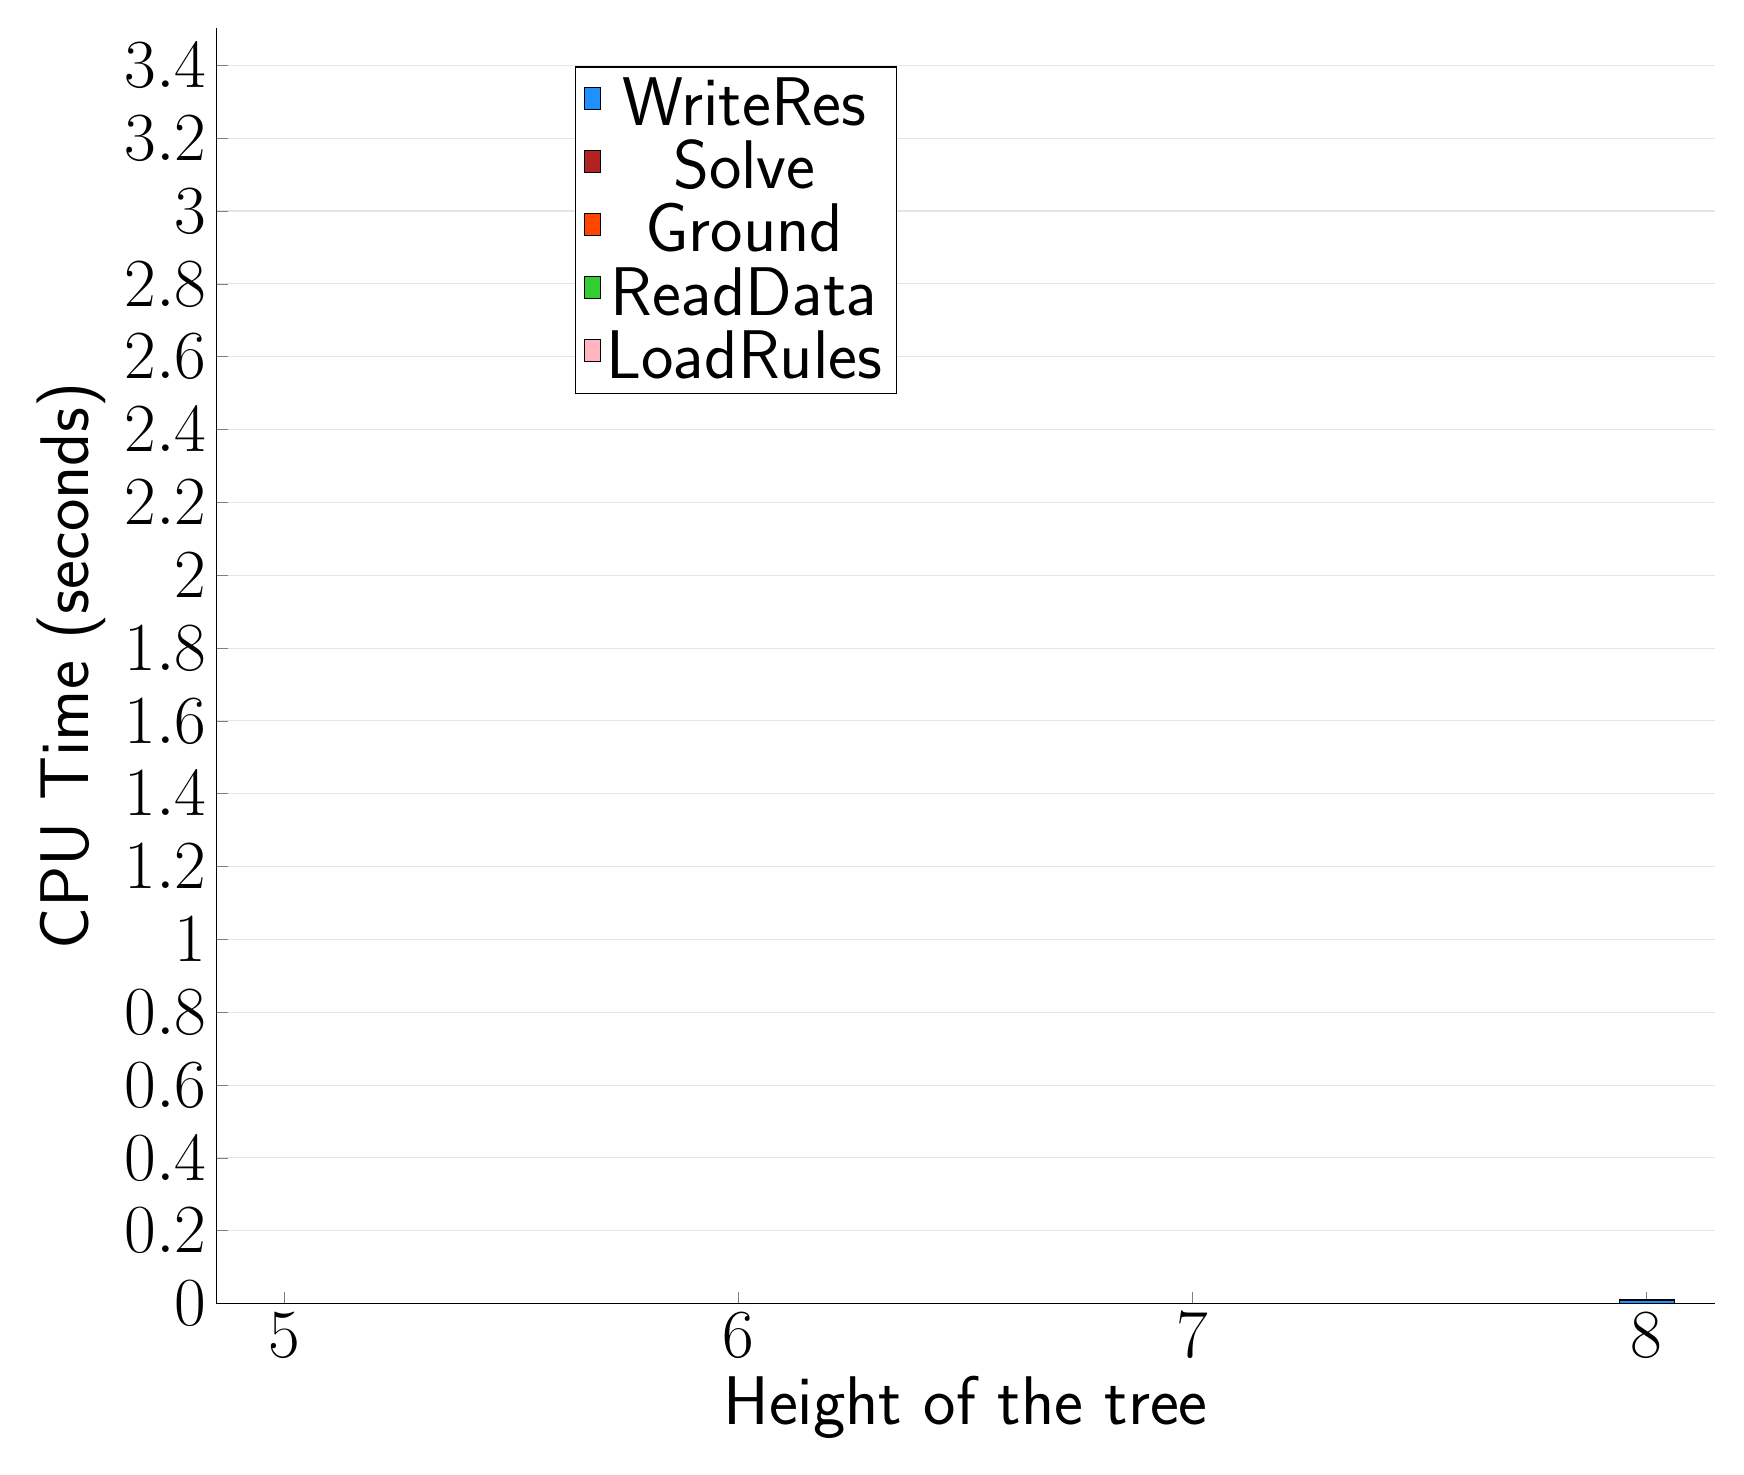
\begin{tikzpicture}
	\begin{axis}[
			ybar stacked,
			width=1.7\textwidth,
			bar width=0.7cm,
			ymajorgrids, tick align=inside,
			major grid style={draw=gray!20},
			xtick=data,
			ymin=0, ymax=3.5020000000000002,
			axis x line*=bottom,
			axis y line*=left,
			enlarge x limits=0.05,
			legend style={
					at={(0.454, 0.97)},
					anchor=north east,
					legend columns=1,
					font=\Huge,
				},
			ylabel={CPU Time (seconds)},
			xlabel={Height of the tree},
			label style={font=\Huge},
			tick label style={font=\Huge},
		]
		\addlegendimage{fill=DodgerBlue, draw=black, line width=0.2pt}
		\addlegendentry{WriteRes}
		\addlegendimage{fill=FireBrick, draw=black, line width=0.2pt}
		\addlegendentry{Solve}
		\addlegendimage{fill=OrangeRed, draw=black, line width=0.2pt}
		\addlegendentry{Ground}
		\addlegendimage{fill=LimeGreen, draw=black, line width=0.2pt}
		\addlegendentry{ReadData}
		\addlegendimage{fill=LightPink, draw=black, line width=0.2pt}
		\addlegendentry{LoadRules}
		\addplot +[fill=LightPink, draw=black, line width=0.2pt] coordinates {
				(5, 0.0)
				(6, 0.0)
				(7, 0.0)
				(7, 0.0)
				(7, 0.0)
				(8, 0.0)
				(8, 0.0)
				(8, 0.0)
			};
		\addplot +[fill=LimeGreen, draw=black, line width=0.2pt] coordinates {
				(5, 0.0)
				(6, 0.0)
				(7, 0.0)
				(7, 0.0)
				(7, 0.0)
				(8, 0.0)
				(8, 0.0)
				(8, 0.0)
			};
		\addplot +[fill=OrangeRed, draw=black, line width=0.2pt] coordinates {
				(5, 0.0)
				(6, 0.0)
				(7, 0.0)
				(7, 0.0)
				(7, 0.0009999999999999998)
				(8, 0.0)
				(8, 0.0)
				(8, 0.0)
			};
		\addplot +[fill=FireBrick, draw=black, line width=0.2pt] coordinates {
				(5, 0.0)
				(6, 0.0)
				(7, 0.0)
				(7, 0.0)
				(7, 0.0)
				(8, 0.0009999999999999998)
				(8, 0.0)
				(8, 0.0)
			};
		\addplot +[fill=DodgerBlue, draw=black, line width=0.2pt] coordinates {
				(5, 0.0)
				(6, 0.0)
				(7, 0.0)
				(7, 0.0)
				(7, 0.0)
				(8, 0.009999999999999997)
				(8, 0.009999999999999997)
				(8, 0.009999999999999997)
			};
	\end{axis}
\end{tikzpicture}

\end{document}
